\documentclass[12pt]{article}

\usepackage{preamble}
\usepackage{hyperref}
\usepackage{algorithmicx}
\usepackage{algorithm}
\usepackage{algpseudocode}

\usepackage[font=small,labelfont=bf]{caption}

\begin{document}

\textbf{Final Project.}

Daniel Yao

EN.580.475

\today

\textbf{Introduction.}

Brawl Stars is a 3v3 mobile game developed by Supercell. A best-of-three match proceeds in two stages: the draft and the gameplay.

First, the game mode (there are six total) is revealed. Two teams, Blue and Red, each independently choose 3 of 97 brawlers to ban. These bans are then revealed. Blue chooses one brawler, Red chooses two brawlers, Blue chooses two brawlers, and then Red chooses one brawler. These brawlers are chosen without replacement so that each team has three brawlers and that these brawlers are unique. The players then play the game mode with their chosen brawlers, and the victor is decided in a best of three contest. Hence, a match is composed of a draft and up to three games.

In the past few years, the competitive community has come to jokingly refer to the game as "Draft Stars", due to the increasing importance of the draft stage over the gameplay stage with the addition of new characters.

I address this draft stage. First, I train three models (logistic regression, random forest, and neural network) to predict the game outcome given a draft. I evaluate these three models and select the best one. I then propose a minimax algorithm to determine the optimal draft strategy using this model. Finally, I address the (many) limitations of my method and draw some conclusions about the state of the game.

\textbf{Methods.}

\textit{Data collection.} The data are taken from a .csv file I logged during the summer of 2024 through BrawlStarsAPI. These data are already preprocessed. Though the data are old, the analysis here is new. In total, there are 5514 games with 82 unique brawlers. I shall only consider these 82 brawlers represented in the data set. All games include at least one top 200 global player, so these games may be regarded as representative of high-level gameplay, where (presumably) skill difference between players is small.

Figure \ref{fig:heatmap} shows the win rate of every brawler against every other brawler in the data set. The heat map is sparse, as expected, because most match ups are not represented in the data.

\begin{figure}[h!]
\centering
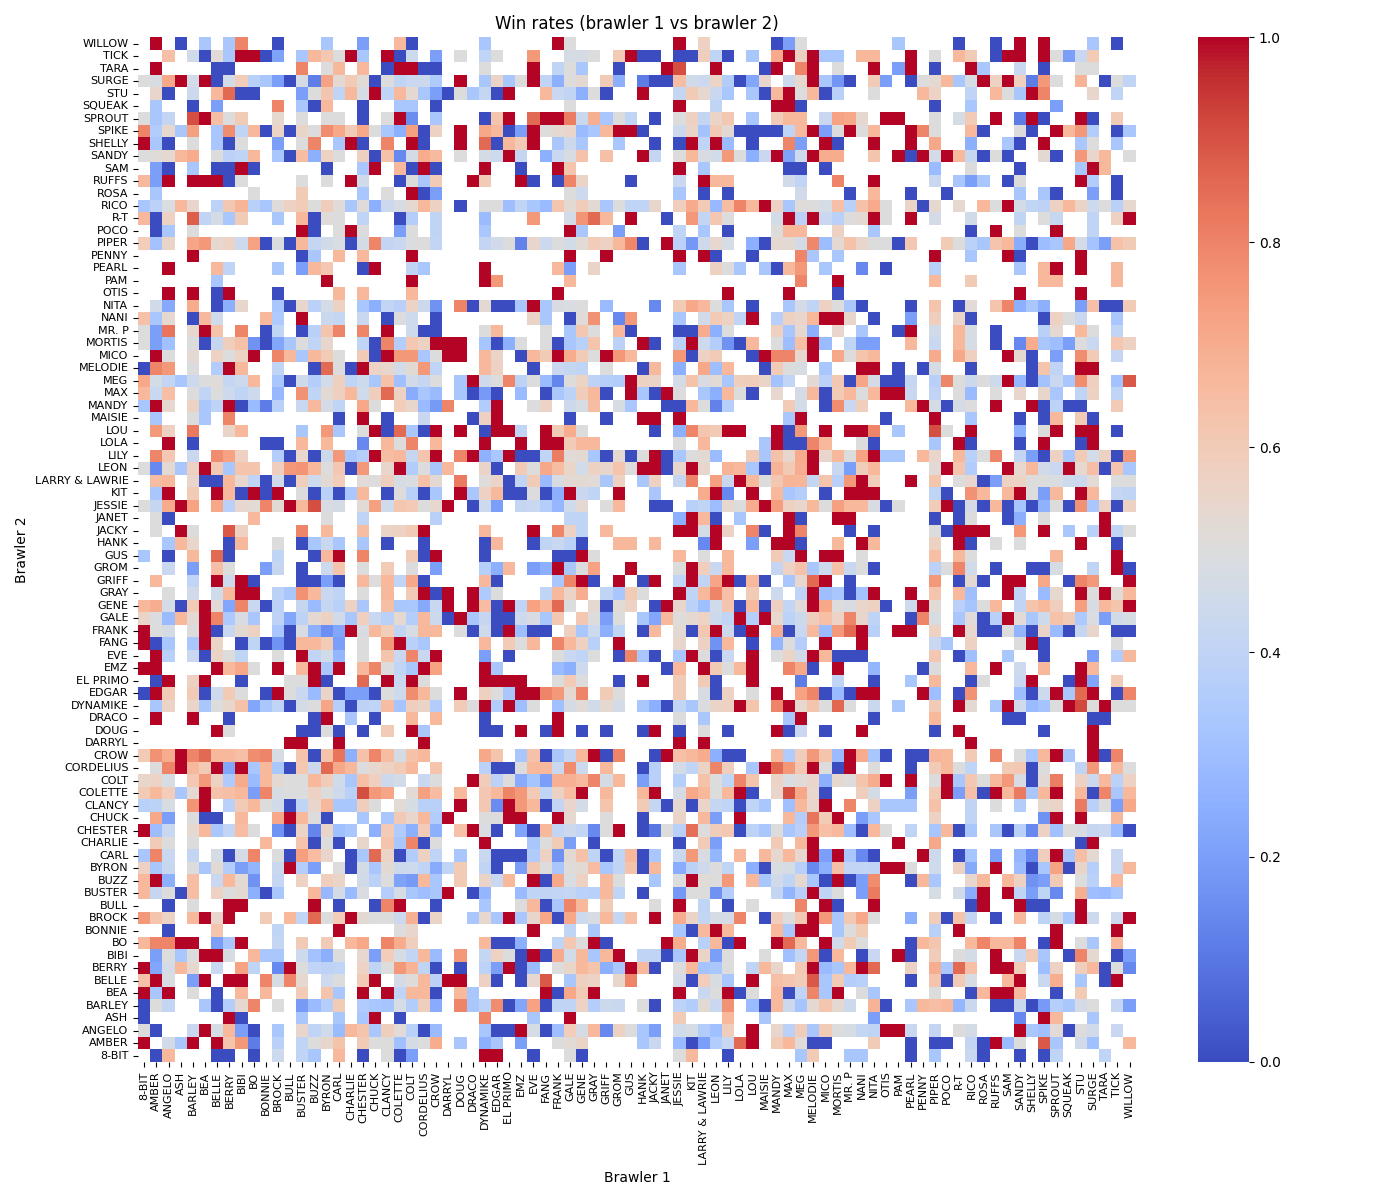
\includegraphics[width=6.5in]{../output/heatmap.png}
\caption{Heatmap with win rates between Brawler 1 vs Brawler 2. The heat map is sparse, as expected, because most match ups are not represented in the data.}
\label{fig:heatmap}
\end{figure}

Since the modes and brawlers are categorical with no meaningful order to these categories, the data are one-hot encoded. There are 6 modes and 82 choices for six players, for a total of 
$$6 + 6(82) = 498$$
dimensions. The brawlers are sorted within each team to respect order invariance within teams.

The data are split 80/20 between training/testing without shuffling. Since it cannot be assumed that the outcome of game 1 is independent of game 2, given a draft, I try to minimize data leakage by keeping games within a match within the same testing/training regime.

\textit{Logistic regression.} A logistic regression classifier is trained with L2 regularization. The operating point is selected to minimize the distance to the top-left corner of the ROC curve.

\textit{Random forest.} A random forest classifier is trained with 20 trees and Gini impurity criterion. The number of trees is determined empirically. It is found that a small model of 20 trees performs the best. The operating point is selected to minimize the distance to the top-left corner of the ROC curve.

\textit{Neural network.} A neural network is trained with two hidden layers of 32 neurons, ReLU activations, sigmoid output, and BCE loss. The number and size of the hidden layers is determined empirically. It is found that a small model of two hidden layers of 32 neurons performs the best. The operating point is selected to minimize the distance to the top-left corner of the ROC curve.

\textbf{Results.}

The training/testing confusion matrices for each of the three models are shown in Figures \ref{fig:lr-cm}, \ref{fig:rf-cm}, and \ref{fig:nn-cm} in the Appendix. The training/testing accuracies, precisions, and recalls are exhibited in Table \ref{tab:performance} Precision and recall remain fairly balanced in both the training and testing sets for all three models. However, these results show that the models grossly overfit to the training data and fail to retain their training performance in the testing regime.

\begin{table}[h!]
\centering
\begin{tabular}{c|ccc|ccc}
    & \multicolumn{3}{c|}{\textbf{Training}} & \multicolumn{3}{c}{\textbf{Testing}} \\ 
    & Accuracy & Precision & Recall & Accuracy & Precision & Recall \\ 
    \hline
    Logistic Regression & 0.66 & 0.67 & 0.66 & 0.56 & 0.57 & 0.56 \\ 
    Random Forest & 0.87 & 0.87 & 0.87 & 0.55 & 0.56 & 0.55 \\ 
    Neural Network & 0.87 & 0.87 & 0.87 & 0.54 & 0.57 & 0.54 \\ 
\end{tabular}
\caption{Training and testing performance. All three models overfit to training data and perform similarly on testing data.}
\label{tab:performance}
\end{table}


The testing accuracies of each of the three models are shown with 95\% confidence intervals (computed as binomial distributions) in Figure \ref{fig:acc}. A baseline positive rate reference is shown, which depicts the accuracy of always predicting the (training set) majority class. All three models perform with roughly 55\% accuracy, which is significantly better than the baseline positive rate at a significance level of $\alpha = 0.05$. The performance between the models is indistinguishable at a sifnificance level of $\alpha = 0.05$.

\begin{figure}[h!]
\centering
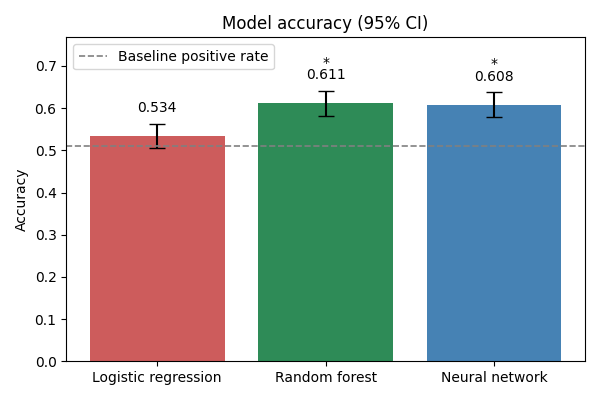
\includegraphics[width=4in]{"../output/acc.png"}
\caption{Testing accuracy. All three models perform significantly better than baseline at $\alpha = 0.05$.}
\label{fig:acc}
\end{figure}

The $R^{2}$s of each of the models for the testing set is shown with 95\% confidence intervals (computed as squared t-distributions) in Figure \ref{fig:r2}. The $R^{2}$ is computed as 
$$R^{2} = 1 - \frac{y^{T}\hat{y}}{y^{T}y},$$
where $y$ is the vector of true labels and $\hat{y}$ is the vector of predicted probabilities. This value roughly corresponds to the proportion of variance explained by the model. The models explain 1-2\% of the total variance, which is significant at a significance level of $\alpha = 0.05$. The performance between the models is indistinguishable at a significance level of $\alpha = 0.05$.

\begin{figure}[h!]
\centering
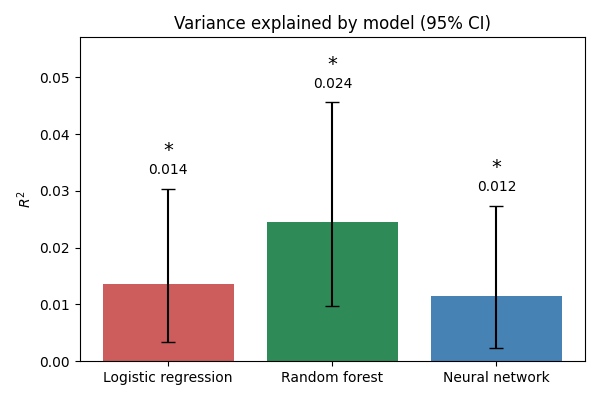
\includegraphics[width=4in]{"../output/r2.png"}
\caption{Testing variance explained. $R^{2}$ is computed as the squared Pearson's correlation between the labels and the predicted probabilties. All three models perform significantly better than guessing at a significance level of $\alpha = 0.05$.}
\label{fig:r2}
\end{figure}

\textbf{Discussion.}

Each of the three models performs better than randomly guessing and explain a non-zero amount of variance. No model achieves very high accuracy, but this is expected because the draft is not the only factor that determines the outcome of a game.

Strong conclusions are hard to draw from these results. There are many confounders at play. Though the outcome of a match can be predicted better than chance from only the draft, there is the possibility that players who are better mechanically are also better draft-wise. Nevertheless, a rough heuristic yields that these data are compatible with the explanation that (at least) 10\% of games are determined entirely by the draft while the other (at most) 90\% of games are determined entirely by mechanics. This roughly matches my experience from playing the game.

Another limiation is that the data only included 5,414 games, while there are 
$$\binom{82}{3,3,76} \big/ 2 = 3,501,618,120$$
total match ups (A vs B is identical to B vs A). As such, almost all possible match ups are not represented in the data set. The models therefore operates almost entirely out of distribution. Nevertheless, the all three of the models are able to generalize to unseen data with better-than-guessing performances.

A final limitation is that the choice of brawlers is very map dependent even within a game mode. To reduce the dimensionality of the state space, I aggregated the maps within each game mode. However, to those familiar with the game, this may not be reasonable. This limitation could be resolved with more data.

\textbf{Application.} 

Now that a model for predicting the outcome of a match given a draft is provided, this model can be used to advise a team how to draft to maximize its victory probability. The minimax algorithm is a deterministic algorithm that finds the optimal strategy to maximize a utility function in a two-player game. The algorithm features two agents, a maximizer and a minimizer, who choose the strategy that maximizes/minimizes the guaranteed utility regardless of the opponent's strategy. The minimax with alpha-beta pruning algorithm is a depth-first search of the action space, which prunes branches that are worse than the previously found maximum/minimum. Formally, the algorithm solves the optimization problem 
$$(A, B) = \arg\max_{a \in \mathcal{A}} \min_{b \in \mathcal{B}} U(a, b),$$
where $A \in \mathcal{A}, B \in \mathcal{B}$ are the actions taken by the maximizer and the minimizer, chosen from their respective action spaces $\mathcal{A}, \mathcal{B}$, and $U$ is the utility function.

In this case, the actions are to select brawlers in accordance to the draft rules, and the utility function is the victory probability predicted by a model. The random forest model is found to work the best for this application. The ban phase is ignored to reduce the state space. The minimax algorithm is described in greater detail in Algorithm \ref{alg:minimax} in the Appendix.

Nevertheless, the state space remains very large, containing 
$$\binom{82}{3,3,76} = 7,003,236,240$$
possible match ups (A vs B is not identical to B vs A). A full-depth search is computational infeasible, but this issue can be resolved by precomputing lookup tables or by parallelization. The focus of this project is not on the minimax algorithm, so the algorithm is only implemented to function, starting from pick $4$. An example draft is shown in Table \ref{tab:draft}, where $(*)$ marks picks that are chosen by the minimax algorithm.

\begin{table}[h!]
\centering
\begin{tabular}{c|ccc|ccc}
    & \multicolumn{3}{c|}{\textbf{Team 1}} & \multicolumn{3}{c}{\textbf{Team 2}} \\ 
    Mode & Pick 1 & Pick $4^{*}$ & Pick $5^{*}$ & Pick 2 & Pick 3 & Pick $6^{*}$ \\
    Bounty & Brock & 8-Bit & Belle & Gene & Max & Bonnie \\
    \hline
    \textbf{Utility} & & 55\% & &  & 45\% & 
\end{tabular}
\caption{Example draft.} Picks marked with $(*)$ are chosen by the minimax algorithm. Utility is measured by predicted victory probability.
\label{tab:draft}
\end{table}

This appears to be a very reasonable draft. Belle and Brock are good against 8-Bit, so it makes sense that they might be on the same team. Moreover, Belle is exceptionally good against Gene, so it makes sense that she should be picked against him.

\textbf{Conclusion.}

In this project, I predict the outcome of Brawl Stars matches given a draft. I demonstrate that a logistic regression, a random forest, and a neural network model each perform significantly better than guessing but they do not perform significantly differently from each other. Moreover, I propose a minimax algorithm to select the optimal draft sequence using these three models, and I demonstrate that this algorithm produces plausible draft sequences.

Each of these models achieve roughly 55\% accuracy and account for only 1-2\% of total variance in testing. Though it is hard to draw conclusions from a small data set, these results do not show that Brawl Stars has become 'Draft Stars'. It still seems that most variance in Brawl Stars is a function of mechanics and not draft.

Possible next steps are to train the same models on more data. With more data, it would be valuable to use the map instead of the game mode as a predictor because the maps within a game mode can be dissimilar. A method to smooth the model or data over unseen match ups would also be valuable so that the model is punished for extreme predictions for mathc ups outside of the training set. Finally, the minimax algorithm could be improved in efficiency (by code optimization and lookup tables), and I could also explore non-ML techniques based on my domain knowledge to augment the utility predictions.

\textbf{Code availability.}

\href{https://github.com/dyao13/580_475_FA25}{github.com/dyao13/580\_475\_FA25}

\newpage \textbf{References.}

Brawl Stars. (2017). Supercell.

Course notes.

Minimax algorithm in game theory. (2023) Geeks for Geeks.

Random forest algorithm in machine learning. (2025) Geeks for Geeks.

\newpage \textbf{Appendix.}

\begin{figure}[h!]
\centering
\begin{center} 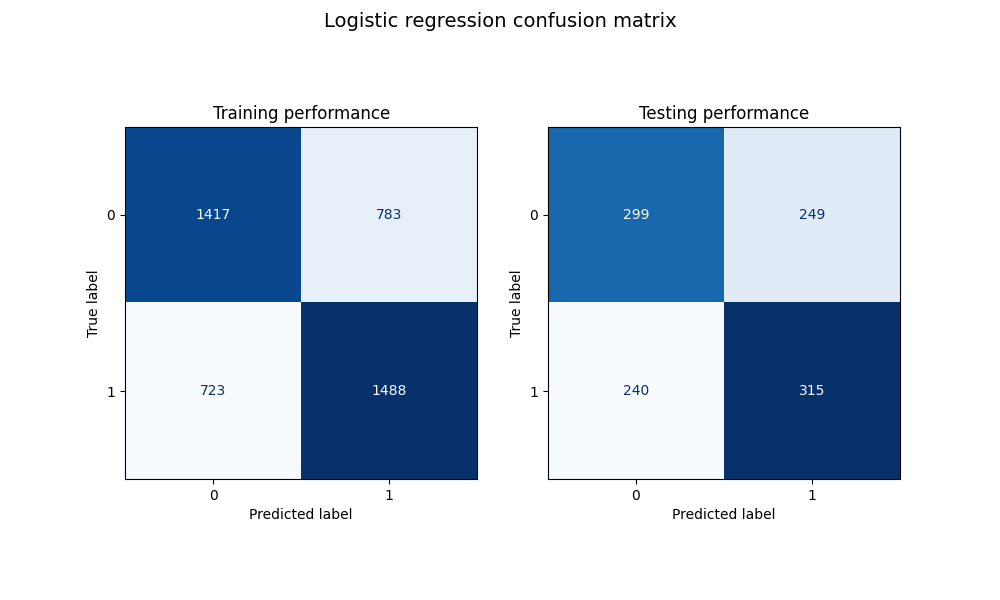
\includegraphics[width=6in]{"../output/lr_confusion_matrix.png"} \end{center}
\caption{Confusion matrix for logistic regression model.}
\label{fig:lr-cm}
\end{figure}

\newpage 

\begin{figure}[h!]
\centering
\begin{center} 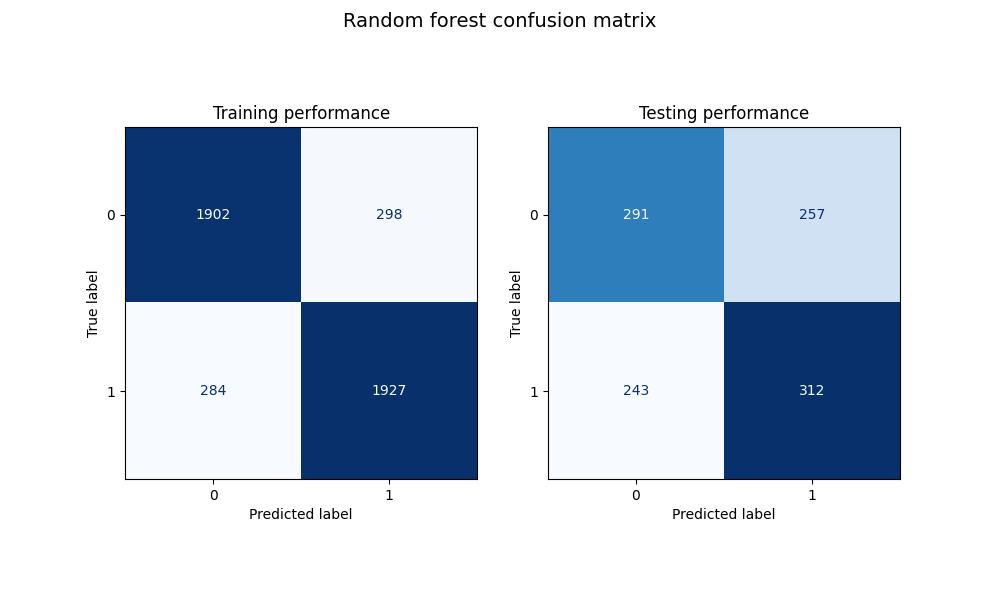
\includegraphics[width=6in]{"../output/rf_confusion_matrix.png"} \end{center}
\caption{Confusion matrix for random forest model.}
\label{fig:rf-cm}
\end{figure}

\newpage 

\begin{figure}[h!]
\centering
\begin{center} 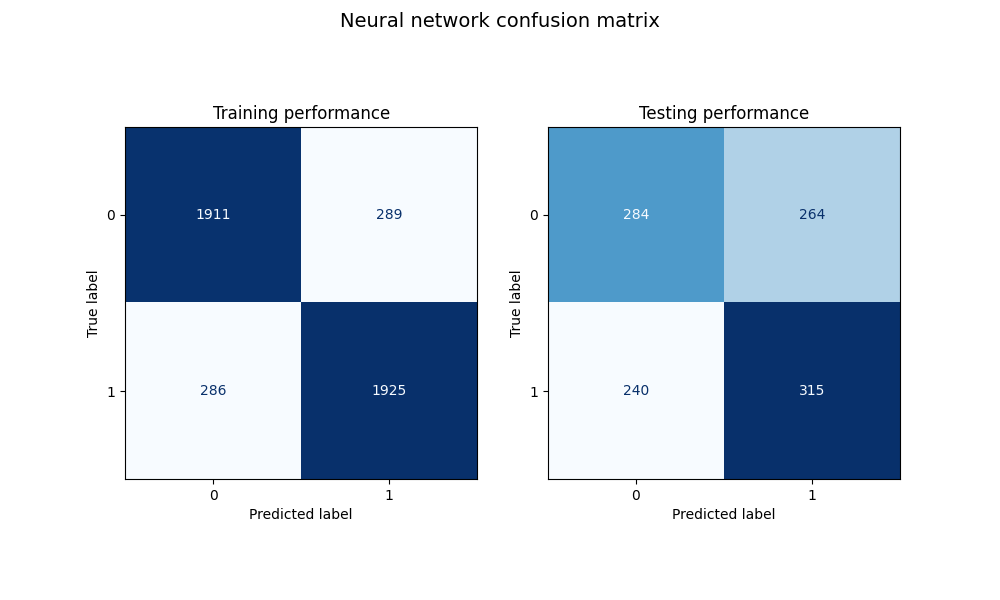
\includegraphics[width=6in]{"../output/nn_confusion_matrix.png"} \end{center}
\caption{Confusion matrix for neural network model.}
\label{fig:nn-cm}
\end{figure}

\newpage
\begin{algorithm}[h!]
\caption{Minimax with $\alpha$–$\beta$ pruning}
\label{alg:alphabeta}
\begin{algorithmic}[1]
\Function{Minimax}{$\text{draft}, d, \alpha, \beta, \text{isMaximizer}$}
    \If{$\textsc{Terminal}(s)$ \textbf{ or } $d = 0$}
        \State \Return $\text{draft}, \textsc{Utility}(s)$
    \EndIf
    \If{\text{isMaximizer}}
        \State $v \gets -\infty$
        \ForAll{$a \in \textsc{Picks}(\text{draft})$}
                \If {$a \cap \text{draft} = \emptyset$}
                    \State $v \gets \max\big(v,\ \textsc{Minimax}(\text{draft} + a,\ d-1,\ \alpha,\ \beta,\ \textbf{false})\big)$
                    \State $\alpha \gets \max(\alpha, v)$
                    \If{$\alpha \ge \beta$} \State \textbf{break}
                    \EndIf
                \EndIf
        \EndFor
        \State \Return $v$
    \Else
        \State $v \gets +\infty$
        \ForAll{$a \in \textsc{Picks}(\text{draft})$}
            \If {$a \cap \text{draft} = \emptyset$}
                \State $v \gets \min\big(v,\ \textsc{Minimax}(\text{draft} + a,\ d-1,\ \alpha,\ \beta,\ \textbf{true})\big)$
                \State $\beta \gets \min(\beta, v)$
                \If{$\alpha \ge \beta$} \State \textbf{break}
                \EndIf
            \EndIf
        \EndFor
        \State \Return $v$
    \EndIf
\EndFunction
\end{algorithmic}
\label{alg:minimax}
\end{algorithm}

\end{document}